\chapter{Background}
\label{ch:background}

% PIZZONE INTRO
In recent years, there has been a growing demand for applications capable of processing high-volume data
streams in real-time~\cite{8-reqs}. These stream-based applications include, among others, financial
algorithmic trading~\cite{streambase-algo}, environmental monitoring~\cite{swissexp} and the real-time
processing of social media events~\cite{social-networks}.  
This research work focuses on the issues arising when the amount of input data
exceeds the processing capabilities of the system. In this scenario, it is necessary to employ
techniques that overcome an overload condition and keep delivering results in a timely fashion. 
The system should gracefully degrade the correctness
of the computed results, following the principle that an approximate result is better than no
result at all. 

Many classes of applications do not require perfect results at all times. Examples are
environmental monitoring and social media analysis. These application domains are the most suitable to be operated
under overload as they are able to tolerate a certain degree of approximation in the results. They deal
with large sets of input data that may require an extremely large amount of processing resources,
possibly beyond what is available to the user. In many cases, it is possible to trade the correctness of
results against a reduction of the cost for the processing infrastructure.

Overload is a particular kind of failure because an excessive amount of data can render a
stream processing system unusable. The management of overload can be achieved mainly with two
techniques: \mbox{load-shedding} and approximate operators. \mbox{Load-shedding} is the process of
deliberately discarding a certain percentage of the input data. The correct execution of load-shedding,
(\ie choosing the right set of tuples to be discarded, can have a great impact on the quality of the computed result).
In addition, it is also possible to reduce the complexity of operators, employing approximate versions
that present a similar semantic but pose a significantly lower computational cost.

%\todo{add outline chapter}

%--------------------------------------------------------------------------------------------------------

\section{Stream-based applications}
\vspace{-10pt}
Traditionally, stream processing has been used in application domains with low tolerance
of failure. Such applications can only produce meaningful results when the processing is carried
out without any loss of data or approximation.
Financial algorithmic trading~\cite{streambase-algo} is a prime example. 
Investment banks, trading on the stock market, need to process a large volume of financial events in
real-time.
Complex algorithms are used to capture the current market situation and to give hints on
profitable trades, exploiting temporary arbitrage conditions. For these applications, the focus is on
efficiency: being able to make a trade even a split second before a competitor is the key to make
profit.
In this scope, the necessity of processing all the available data is evident because a wrong choice
based on approximate data could lead to financial loss.

On the other hand, there are some classes of applications that are able to operate correctly even when
not all the data can be processed. In many cases, a certain degree of failure in the system is
tolerable and does not prevent the application from producing meaningful results.

We will describe two broad classes of applications that can use an approximate result approach.  
The first class are \emph{global sensing infrastructures}~\cite{senseweb,gsn,irisnet}, which are
concerned mostly with sensor data, developing a worldwide infrastructure in which different classes of
sensors can be connected and accessed through a common interface. They allow users to process data
streams generated by different sensor networks.
 
A second class that can benefit from this approach are applications for \emph{real-time
processing of social media events}. These applications analyse the constant stream of user generated
content, extracting useful information from it. It is possible to process user-generated data
streams, for example from Twitter, to understand how the public reacts to a certain product launch or
event~\cite{twitter-sentiment,twitrratr}, identifying trends as they
arise~\cite{twitter-stocks,twitter-sentiment-1}. It also possible to exploit the locality
information disclosed by the users in order to identify differences in lifestyle and
preferences, as done by FourSquare~\cite{foursquare-wsj,foursquare-rude}.
\vspace{-15pt}
%--------------------------------------------------------------------------------------------------------
\subsection*{Environmental Monitoring}
\label{envmon}
%\vspace{-10pt}
The first domain of applications that we will take into consideration are related to large-scale
scientific sensing, in particular we will describe projects dealing with large-scale environmental
monitoring.  In recent years, the availability of cheap micro-sensing technology has unleashed sensing
at an unprecedented scale. We can expect in the future to see everything of material significance being \emph{sensor-tagged} and report its state or location in
real-time~\cite{irisnet,qpsn,stream-processing-challanges}. At the present time, a great number of
large-scale sensing projects are being developed and we can expect even more to come soon into
place~\cite{earthscope,neon,casa-lead,swissexp}.

One area in which large-scale sensing has flourished is \emph{environmental monitoring}. The growing
concern about climate change has brought a lot of attention to environmental studies. Many
large-scale sensing projects have been launched to understand better the behaviour of many natural
processes.
Examples of such efforts are, for instance, the Earthscope~\cite{earthscope} and the Neon~\cite{neon}
projects.

Earthscope is a multi-disciplinary project across earth sciences to study the geophysical structure and
evolution of the American continent. It uses a large number of sensors geographically distributed over
the whole continent to answer some of the outstanding questions in Earth Sciences by looking deeper, at
an increased resolution, and integrating diverse measurements and observations.~Thousands of geophysical
instruments measure the motion of the Earth's surface, record seismic waves and recover rock samples from
depths at which earthquakes originate. All the collected data is freely available, and a large community
of scientists is conducting several multidisciplinary studies based on it. Examples of sensing
projects within Earthscope include the constant monitoring of the San Andreas fault and the Plate Bound
Observatory, which collects information about the tectonic movements across active boundary zones.
NEON stands for National Ecological Observation Network. This project aims at creating a new national
observatory network to collect ecological and climatic observations across the United States. It is an
example of a continental-scale research platform for discovering and understanding the impact of climate
change, land-use change and invasive species on ecology. It is the first observatory designed to detect
and enable forecasting of ecological change at continental scales over multiple decades. Obtaining this
kind of data over a \mbox{long time} period is crucial to improving ecological forecast models and will
greatly help understand the effects of human interference on climate. These are just
two examples of large-scale monitoring projects, and many others already exists or will be started in the
near future~\cite{testban,skysurvey,neon,usvo}.

Environmental sensing is a natural application for stream processing systems because a continuous flow of
measurements are generated by a large number of sensors. Stream processing offers an intuitive and
flexible paradigm to harness such a high volume of data. It also gives the possibility of obtaining a
real-time picture of the measured phenomena, enabling quick reaction to possibly disruptive events. The
core components of these projects are sensing stations, which are geographically distributed and
frequently subject to harsh conditions. In such scenarios, the failure of sensing devices is common and
often their replacement is problematic. Long running continuous queries need to be able to handle some missing
data, adapting to the new conditions and reporting the achieved quality of processing. To collect and
process all data at all times remains infeasible, and it is important for the computing backbone of such
projects to be able to withstand a certain degree of failure within the system~\cite{dependable-is-sensing}.
% 
% I will now present a more specific example of infrastructures aiming at supporting large-scale sensing
% projects.  The first is concerned with meso-scale weather monitoring, while the second focuses on the
% collection of data from environmental sensors in a more general purpose fashion. Both project could take
% advantage from my research, by enabling them to produce results in real-time and to better operate in the
% occurrence of failure due to an excessive amount of input data.
\paragraph{Distributed Collaborative Adaptive Sensing.} Meso-scale weather events, such as tornadoes and
hurricanes, cause a large number of deaths and a great deal of damage to infrastructures every year.
Being able to understand and predict when these hazardous weather conditions will occur can greatly
mitigate their consequences.

In this regard, the National Science Foundation has recently established the center for
\textit{Collaborative Adaptive Sensing of the Atmosphere (CASA)}~\cite{casa}. Its goal is to
enhance the current infrastructure of long-range weather observing radars with a large number of small
solid-state radars in order to increase the sampling resolution throughout the entire
troposphere.
Although current \mbox{long-range} radar technology allows the coverage of large areas with a relatively
small number of devices, these are not able to measure correctly the lowest part of the atmosphere in
areas far away from the radar. This is due to the Earth's curvature and terrain-induced blockage.  This
new sensing paradigm, based on a large number of smaller devices, is referred to as \emph{Distributed
Collaborative Adaptive Sensing~(DCAS)}. Distributed refers to the use of numerous small and inexpensive
radars, spread densely enough to measure the area fully, even at lower altitudes at which the traditional
approach fails.
Collaborative refers to the coordination of multiple devices that cover overlapping areas to increase
the resolution and the precision of the measurements compared to a single radar. Adaptive refers to the
ability of the infrastructure to dynamically adjust its configuration based on the current weather
conditions and user needs.
Similar to CASA is the \emph{Linked Environments for Atmospheric
Discovery~(LEAD)}~\cite{lead}. It gives scientists the tools with which they can automatically spawn
weather forecast models in response to real-time weather events in a desired region of interest. It is a
middleware that facilitates the adaptive utilization of distributed resources, sensors and workflows.
While CASA is primarily concerned with the reliable collection of the data, LEAD is the backbone
processing infrastructure. It allows the automation of time consuming and complicated tasks associated
with meteorological science through the creation of workflows. The workflow tool links data management,
assimilation, forecasting and verification applications into a single system. Weather information is
available to users in real-time, not being restricted to pre-generated data, which greatly expands
analysis capabilities.

The integration of these two systems offers a useful infrastructure to atmospheric
scientists~\cite{casa-lead}.  First of all, it allows meteorologists to interact directly with data from
the instruments as well as control the instruments themselves. Unlike traditional forecasting
approaches, it allows the establishment of interactive closed loops between the forecast analysis and the
instruments. This sensing paradigm, based on numerous input devices and the possibility of directly
feeding their data into a forecasting model, is changing the way meso-scale weather events are detected
and will help mitigate their impact. Stream processing has the potential of enhancing the CASA/LEAD
infrastructure, extending its real-time monitoring capabilities.
% In this infrastructure, when implemented
% at larger scale, failure is going to be the common case. CASA is built from small weather stations, and
% it is designed to withstand failure at the sources and to reconfigure at run-time~\cite{casa}. This means
% that during long running queries, the backbone processing system is likely to be affected by failure at
% the sources and experience variations in the quality of the results.  For these reasons, this scenario
% would be a prefect test-bed onto which exploring ways to operate a large-scale monitoring system under
% constant partial failure, while constantly measuring the achieved quality-of-service.

% \paragraph{The Swiss Experiment} Another example of large-scale environmental sensing project is
% represented by the Swiss Experiment~\cite{swissexp}. The aim of the project is to enable effective
% real-time environmental monitoring through wireless sensor networks and a modern, generic
% cyber-infrastructure. It is a collaborative projects with many contributions on different scientific
% and technological aspects.
%  Within the scope of the project, a new wireless sensor network technology has been developed, called
% SensorScope~\cite{sensorscope}. This is an out-of-the-box environmental monitoring infrastructure based
% on inexpensive wireless sensor nodes. SensorScope is both a hardware and software architecture. It
% falls into the category of time-driven networks, as the stations intermittently transmit environmental
% data to a sink, which in turn make the received data available through a number of interfaces. It has
% been deployed and tested in many occasions, being one of the fundamental building block employed in the
% project. It was used to monitor the quality of the water in the Le Boiron de Morges river, on Le Genepi
% rock glacier, to monitor dangerous mud streams, and on the Grand St.  Bernard pass, to obtain a very
% precise map of evaporation of the area.
%  PermaSense~\cite{permasense} is another technological effort within the project. It aims at the
% development of an innovative sensor infrastructure for automated, unattended long-term data acquisition
% in the extremes of high-alpine regions. The goal is to investigates the effect of permafrost in
% high-alpine environments.
%  All the data gathered by the project is made available through a number of interfaces like GoogleMaps
% and SenseMap~\cite{sensemap}. The acquisition and storage of the data is also performed in different
% ways. It is saved in a wiki, in comma separated values files, even though the most interesting way is
% through the GSN (Global Sensor Networks).  This is a database software middleware designed to
% facilitate the deployment and programming of sensor networks. Large-scale, long-running monitoring
% tasks like the ones in the aims of the Swiss Experiment are likely to experience failure, either at the
% sources and in the distributed backbone processing infrastructure. GSN, the tool employed for
% \mbox{real-time} data mining within this project, reacts to failure by simply releasing the associated
% resources and continuing the processing without them~\cite{gsn-book}. This behaviour could be improved,
% by introducing the ability of introducing quality-awareness in its processing. Extending GSN in this
% regard, would allow it to better operate in hostile environments characterized by a high occurrence of
% failure. This would enhance its capabilities, providing users with a better understanding of
% approximate results and the behaviour of the system.


% \begin{figure}[b!] \centering \includegraphics[scale=0.4]{img/swissex-overview.jpg} \label{img:swissex}
% \caption{Outline of the SwissEx infrastructure} \end{figure}


% \subsubsection*{Astrophysics} 
\label{sec:astro} 
%\notemf{I find the structure here to be a little confusing. Some options: a) eliminate astrophysics b) talk of swiss
%experiment in the introduction of the paragraph, as it is a more general purpose experiment c) leave it like this d)
%your say?}

\begin{structure}
	\item Application of StreamGlobe, explained in Section \ref{sec:streamglobe}
\end{structure}

StarGlobe: Grid-Based Data Stream Processing in e-Science \cite{starglobe-grid}

%--------------------------------------------------------------------------------------------------------
\subsection*{Real-time Social Media Analysis}

Social networks have experienced a large growth over the past years~\cite{flickr-growth}, changing the
Internet landscape by shifting the balance of the available information towards user-generated content.
Numerous sites allow users to interact and share content based on social links. Users of these networks
often establish hundreds or even thousands of social links with other users, constantly reshaping the
social graph~\cite{fb-interactions}.
Users share photos~\cite{flickr, facebook}, videos~\cite{youtube}, status updates~\cite{twitter} and
locations~\cite{foursquare}, providing a continuous stream of valuable information for researchers and
companies. 
Social media analysis has become an essential tool for online marketing, and many tools have been
developed to help discovery and to reach new potential customers~\cite{wildfire, brandwatch}. The
possibility to target specific segments of the online population with customised advertisements allows
companies to increase their return on investment and users to avoid unwanted communication.
Furthermore, by analysing Twitter streams, it is possible to predict in real-time the evolution of
numerous phenomena, such as the spreading of diseases~\cite{mappyhealth} or the fluctuation of stock
quotes~\cite{twitter-stocks}. Other applications analyse keywords in status updates to determine the
public sentiment towards a certain topic, brand or public figure~\cite{socialmention, twendz, tweetfeel}.
The diffusion of user-generated content through a social network is referred to as a \emph{social
cascade}. The next section describes social cascades and explains why their prediction can be useful for
the correct allocation of resources in content distribution networks.
% 
% \section{Twitter Analisys Tools}
% 
% Many tools have been developed to extract information from Twitter statuses. Th
% 
% 
% \emph{Social Mention}~\cite{socialmention} is a tool that allow the tracking of certain keywords across
% over 80 social networks. It monitors the status update streams produced by users of the major social
% networks and it filters only those containing a certain keyword. It provides a list of all statuses
% together with a number of statistics. It is possible for instance to monitor how many people mention the
% keyword, what sentiment are expressed in the statuses, what other keywords appear the most together with
% the status. One of the aims of this tools is to help marketers to assess the perception of a brand or to
% measure the impact of media campaign. 
% \emph{Strength} is the likelihood that a certain brand is being discussed on social media, given by
% phrase mentions within the last 24 hours divided by total possible mentions. \emph{Sentiment} is the
% ratio of mentions that are generally positive to those that are generally negative. \emph{Passion} is a
% measure of the likelihood that individuals talking about a brand will do so repeatedly. \emph{Reach} is 
% a measure of the range of influence. It is the number of unique authors referencing a brand divided by
% the total number of mentions. 
% 
% 
% 
% 			\bul{Overview of trends in social networks}
% 			% \incite{social-networks}
% 
% 			\incite{storm} 
% 
% 			\bul{Twitter Analysis Tools}
% 			%\incite{socialmention}
% 			\incite{twitrratr}
% 			\incite{twitter-sentiment}
% 			\incite{ubervu}
% 			\incite{twendz}
% 			\incite{tweetfeel}
% 
% 			\bul{FourSquare Articles}
% 			\incite{foursquare-wsj}
% 			\incite{foursquare-rude}	
% 
% 			\bul{Papers on Twitter sentiment analysis}
% 			\incite{twitter-stocks}
% 			\incite{twitter-sentiment-1}
% 			\incite{twitter-sentiment-2}
% 			\incite{twitter-sentiment-3}
% 			\incite{twitter-sentiment-4}
% 			\incite{twitter-sentiment-5}
% 
% 			\bul{Papers on Social Casacades}
% 			\incite{buzztraq}
% 			\incite{socialcascade-flickr}
% 			\incite{socialcascade-salvo}
% 
% 
% % social cascades
\paragraph{Social Cascades.} One interesting application of social media real-time analysis is the
possibility of predicting social cascades. A \emph{social cascade} is the phenomenon generated by the
repeated sharing of a certain content over an Online Social Network (OSN). One person discovers an
interesting piece of information and shares a link to it with a few friends, who share it themselves and
so on. When content is considered interesting by a community, it starts being shared over and over again,
possibly reaching a large number of hits in a short period of time~\cite{socialcascade-flickr}. Due to the
characteristics of social networks, this process mimics the spread of an epidemic~\cite{buzztraq}.
Initial studies about this phenomenon date back to the 1950s, with the theory
of Diffusion of Innovation~\cite{diffusion-innovation}. It is only now though, with the wealth of
information shared through OSNs, that is possible to study social cascading in much more detail.

More formally, a user \emph{Bob} is reached by a social cascade when he receives a certain content
\emph{c} and:
\begin{enumerate}
\singlespacing
	\item User \emph{Alice} already posted content \emph{c} before user \emph{Bob}; and
	\item There is a social connection between users \emph{Alice} and {Bob}.
\end{enumerate}
\paragraph{Social Cascading in Twitter.}
The diffusion of links through Twitter can be used to understand better what a social cascading tree
looks like. Twitter is a micro-blogging website on which users can share a short message of maximum 140
characters with other users called ``followers''. In this particular social network, it is also possible
to characterise cascades further into two main groups: R-cascades, for which the
flow of URLs is constrained to the follower graph and
RT-cascades~\cite{outweeting}, for which the follower graph is disregarded and
the who-credits-whom data from the retweets is used.

R-cascades occur when a certain content is shared by direct followers. More formally, we can
say that an L-cascade is the graph of all users who tweeted about a certain content \emph{c}. A cascade
link is formed when (1) Users \emph{Alice} and \emph{Bob} shared content \emph{c}, (2) User
\emph{Alice} posted \emph{c} before user \emph{Bob}, and (3) User \emph{Bob} is a follower of user
\emph{Alice}.

Instead, RT-cascades do not only take into account direct connections but also the
possibility of crediting certain content to a user even without being a direct follower. If user
\emph{Bob} wants to give credit to user \emph{Alice} for certain content, he prepends his new tweet
with the conventional \emph{RT @Alice} tag followed by the original tweet. In this way, \emph{Bob} gives
direct credit to \emph{Alice} for the content of the tweet even without being a direct follower. This
phenomenon is known as ``retweetting''~\cite{retweet}. More formally, we can say that an RT-cascade
\emph{R(c)} is the graph all the users who have retweeted content~\emph{c} or have received credit for
it.
A cascade link is formed when (1) User \emph{Bob} tweeted about content \emph{c}, (2) User \emph{Alice}
tweeted about content \emph{c} before user \emph{Bob}, and (3) User \emph{Bob} credited user \emph{Alice}
as the original source of the content.
\vspace{-0.5cm}
\paragraph{Impact of Social Cascades on CDNs.}
% CDN
It is difficult to predict where and when certain content will become popular.
Many content providers rely on Content Delivery Networks (CDNs) to distribute their content across
multiple geographic locations in order to enhance the availability of their content to their users. The
choice of \emph{what} content to replicate, \emph{where} and for \emph{how long} is crucial to the
reduction of the costs associated with the use of a CDN. Being able to predict the popularity of certain
content is needed for the correct provisioning of resources. For example, it has
been found that the top 10\% of the videos in a video-on-demand system account for approximately 60\% of
accesses, while the rest of the videos (\ie the 90\% are the tail) account for
40\%~\cite{buzztraq}.

An attempt to characterise the spread of social cascades focuses on improving the caching of
content, exploiting the geographic information from the cascades~\cite{socialcascades-salvo}.
This approach leverages the observation that a social cascade tends to propagate in a geographically
limited area, because social connections typically reflect real life relationships. It is
also likely that a video spoken in a particular language would tend to propagate within the national
borders of a country, in which that language is native. Based on an analysis of a corpus of 334 millions messages
shared on Twitter, extracting about 3 millions single messages with a video links, it was found that
about 40\% of hops in social cascades involve users that are, on average, less than 1,000 km away from
each other.

% 

%--------------------------------------------------------------------------------------------------------

\section{Query Languages}
\label{sec:querymod}

In a DSPS, data is continuously pushed into the system in the form of streams. These are real-time,
continuous, ordered sequences of data items. Streams have different characteristics than traditional
relations in a DBMS, and the way of expressing queries in a DSPS has to take these differences into
account. Streams can be unbounded but queries are usually issued over a recent snapshot of the data
stream, which is referred to as \textit{window}. A query language for data streams must be capable of
operating over windows of data, should be extensible in order to support custom user operators, and
simple enough to enable the easy specification of complex queries. 

Three query paradigms have been proposed for streaming data~\cite{dsm-issues}. The first and
most adopted is the \textit{relational streaming model}. It comes from the DBMS world and is
usually implemented as an SQL-like language. It provides the syntax to express windows over data streams,
similarly to the extensions introduced in SQL-99. A query describes the results in a declarative way,
giving the system the flexibility of selecting an optimal evaluation procedure for producing the desired
answer. Examples of languages employing this model are CQL~\cite{cql}, StreamSQL~\cite{streamsq} and SPADE~\cite{ss-spade}. 

Another method for expressing queries is through \textit{procedural streaming languages}. In this
paradigm, the user constructs queries in a graphical way, having maximum control over the exact series of
steps by which the query answer is obtained. In this model, operators are depicted as boxes and arrows
represent the data streams flowing through them, thus taking the name of \textit{boxes-and-arrows} model.
One drawback of this model is the difficulty of expressing complex query plans because the diagram
describing a query can become intricate. Aurora~\cite{aurora} and Borealis~\cite{borealis-design} are
examples of systems employing this query model.

The third model for expressing queries is the \textit{object-oriented streaming paradigm}. In this
approach, the query elements are modeled in a hierarchical way, taking inspiration from the
object-oriented programming world. In Cougar~\cite{cougar-adt}, for example, sources are modeled as ADTs
(Abstract Data Types), exposing an interface consisting of a sensor's signal processing methods. A discussion of
query languages and practical issues on building a stream processing system can be found
in~\cite{design-principles}.

The next sections present more details on the two main models for expressing queries in a
stream processing system: the \emph{continuous query language} and the \emph{boxes-and-arrows}
representation.

\subsection*{CQL: Continuous Query Language}
\label{sec:cql}

The Continuous Query Language~\cite{cql} is a declarative language for expressing continuous queries
over streams of data. It has been introduced as part of STREAM (Stanford Stream Data
Manager)~\cite{stream} and has become one of the de facto standards in stream processing. It is an
SQL-like language designed to work on streams as well as with relations and to allow an easy conversion
among them. It extends SQL, introducing semantics to enable queries to be issued over streams of data. A detailed description of the
more formal aspects of the language can be found in~\cite{cql-foundation}. 

To better illustrate the main concepts in CQL, let us consider a \textit{temperature monitoring} query.
The purpose of such a query is to detect if the temperature in any room of a building rises above a
certain threshold. If a room becomes too hot, the system detects it and reacts by switching on the local
air conditioning unit. In this scenario, all rooms are equipped with thermal sensors.
These are connected to a stream processing system, which is able to control the air conditioning unit.
The thermal sensors sample the temperature in the room every minute, sending these readings, together with
their room id and timestamp, to the stream processing system. This executes a simple query, filtering
all tuples with a temperature reading above a certain threshold (\eg $T>=30$). When the system
detects that a room is too hot, it switches on the air conditioning unit in that room. 
\subsubsection*{Data Types}

The two core data types manipulated by CQL are \textit{streams} and \textit{relations}.

\begin{definition}[Stream]{A stream S is a potentially infinite bag (multiset) of elements $\langle s,
\tau \rangle$, where $s$ is a tuple belonging to the schema of $S$ and $\tau
\in T$ is the timestamp of the element.}
\end{definition}

Timestamps are not part of the schema of a stream, and there can be zero, one or more elements with
a given timestamp in a stream. The number of elements with the same timestamp in a stream is finite but
unbounded.
In CQL the data part of a stream element is referred to as a \textit{tuple}. There are
two classes of streams: \textit{base streams}, which are the input of the system, and \textit{derived
streams}, which are intermediate streams produced by operators. 

\underline{\textsc{Example}}: In our temperature monitoring scenario there would be only one base stream
with a schema: \textsc{RoomTmpStr(RoomID, RoomTmp)}. Attribute \textsc{RoomID} identifies the room where
the sensor is located, while \textsc{RoomTmp} contains the current detected temperature. 

\begin{definition}[Relation]{A relation R is a mapping from each time instant
$\tau$ to a finite but unbounded bag (multiset) of tuples belonging to the
schema of R.}
\end{definition}

A relation $R$ defines an unordered multi-set of tuples at any instant in time $\tau \in T$,
denoted as $R(\tau)$. The difference between this definition and the one used in databases is that, in
the standard relational model, a relation is simply a set of tuples with no notion of time. 

\underline{\textsc{Example}}: In our scenario, a relation is created from the base stream of
temperature readings through a time-window operator. It is a snapshot of all readings received within the last
minute. The concept of windows over streams will be explained in the next paragraph.

\subsubsection*{Operator Classes}
\begin{figure}[b]
\centering
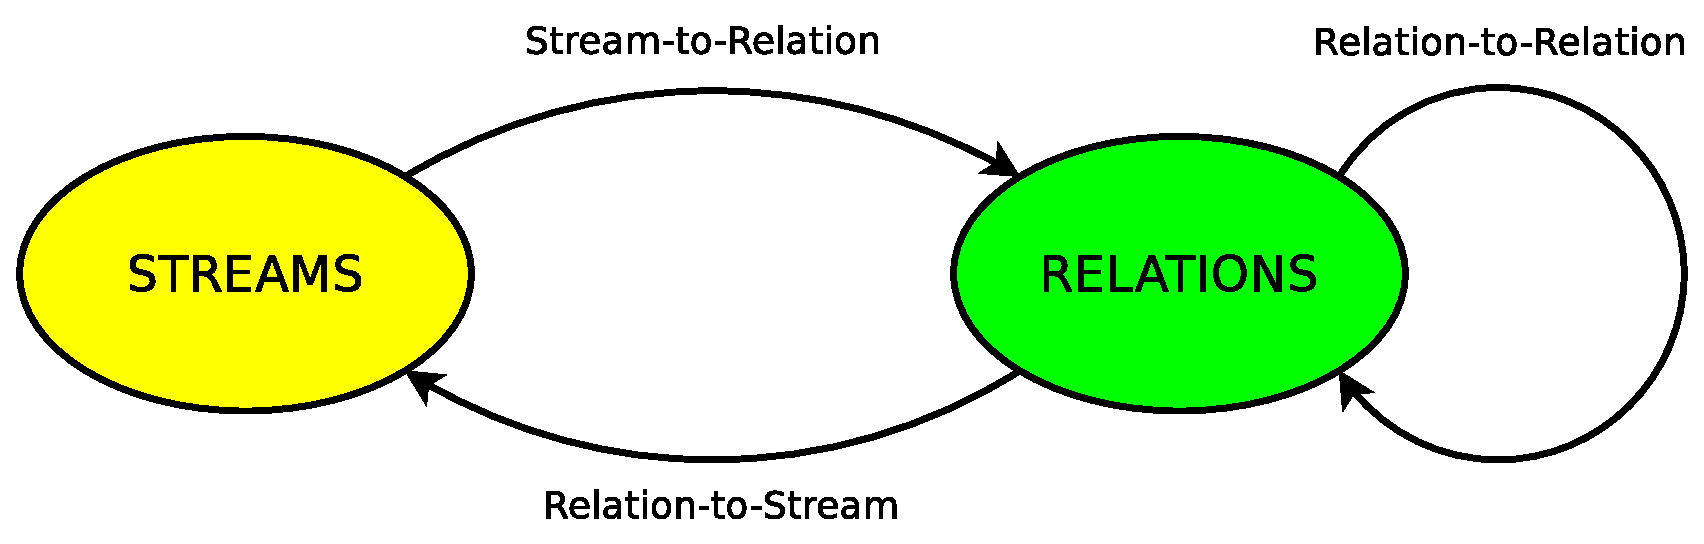
\includegraphics[width=0.8\textwidth]{img/tesi/cql_ops} 
\caption{Interaction among the three classes of operators in CQL.}
\label{fig:cql_ops}
\end{figure}
CQL employs three classes of operators to process stream data. First is the \textit{Stream-to-Relation}
operator, which creates a snapshot of a stream. After a finite bag of tuples has been
obtained, it employs \textit{Relation-to-Relation} operators, which are equivalent to the ones employed in
a traditional DBMS. Finally, there are \textit{Relation-to-Stream} operators to create streams from
newly computed relations. Figure~\ref{fig:cql_ops} shows the interaction between these classes of
operators. 

\paragraph{Stream-To-Relation} operators are used to isolate a subset of a stream, or snapshot, so that
one or more relation-to-relation operators can act on it. All the operators in this class are based on
the concept of a \textit{sliding window} over a stream. This contains, at any point in time, a
historical snapshot of a finite portion of the stream. 

Three kinds of window operators exist in CQL: time-based, tuple-based and partitioned. A
\textit{time-based} window contains all the tuples in the stream that have timestamps within the
specified boundaries. For example, it could hold all the tuples that have arrived in the past minute. In
a \textit{tuple-based} window, instead, the number of tuples is specified and fixed so that it only
contains the last $N$ tuples of the stream. A \textit{partitioned} window is a special kind of the
tuple-based window. It allows the user to specify a set of attributes as a parameter, splits the
original stream based on these arguments, similarly to the SQL GroupBy statement, and computes a
tuple-based window of size $N$ independently creating a number of substreams.

\textit{Sliding Windows} produce a snapshot of a stream based on two parameters: the \textit{window size}
and the \textit{sliding factor}. Once the window is triggered, it outputs all the tuples that it
contains but it does not discard them all. The sliding factor determines a strategy to hold some tuples
in the window so that they can be used in the next iteration. A tuple-based window, for example, can be
set to trigger every 5~tuples with a slide of 1. Every time that it reaches 5 tuples, it outputs all of
them but retains the 4~most recent tuples for the next iteration. A time-based window can be set to
trigger every five minutes with a sliding factor of 1~minute. At every iteration, it outputs all the
tuples that have arrived in the past 5 minutes, retaining all tuples from the past 4 minutes. 

\paragraph{Relation-To-Relation} operators are derived from the traditional SQL relational model. They
perform the bulk of the data manipulation and are equivalent to canonical SQL operators. In this
category, we find, for example, \textsc{Select, Project} and other familiar operators. A stream is
converted into a relation by a window operator, then processed by a relation-to-relation operator and finally output by
a relation-to-stream operator.
      
\underline{\textsc{Example}}: Consider the following query for our temperature monitoring scenario:

\tab \textsc{Select *} \\
\tab \textsc{From RoomTmpStr[Range 5 Min]} \\
\tab \textsc{Where Tmp > 30} 

This query is composed of a stream-to-relation time-window operator, followed by a relation-to-relation
operator performing a projection. The output is a relation that contains, at any time, the set of all
temperature readings received by the system in the past five minutes with temperatures greater than 30
degrees Celsius. 

\paragraph{Relation-To-Stream} operators convert the result of relation-to-stream operators back into a
stream. Three kinds of such operators exists in CQL: \textit{IStream, DStream} and \textit{RStream}.

1. \textbf{IStream} (for ``insert stream'') outputs only the new tuples that have been generated since
the last execution. It compares the current output of the preceding relation-to-relation operator and
outputs all the tuples that are present in the current input but not in the previous one. Informally, it
inserts new tuples into the stream. Formally, the output of \textit{IStream} applied to a relation $R$
contains a stream element $\langle s, \tau \rangle$ whenever tuple $s$ is in $R(\tau)-R(\tau-1)$. Assuming
$R(-1)=\emptyset$, we have: %XXX: fix parentesis

\begin{center}
	$IStream(R) = \bigcup_{\tau>=0}\Big[(R(\tau)-R(\tau-1))\times\{\tau\}\Big]$ %fix union
\end{center}

2. \textbf{DStream} (for ``delete stream'') outputs only tuples that have disappeared since the last
execution. It compares the current output of the preceding relation-to-relation operator and
outputs all the tuples that were present in the previous input but not in the current one. Informally,
it generates the stream of tuples that have been deleted from the relation. Formally, the output of
\textit{DStream} applied to a relation $R$ contains a stream element $\langle s, \tau \rangle$ whenever tuple $s$ is in
$R(\tau-1)-R(\tau)$. %XXX: fix parentesis

\begin{center}
	$DStream(R) = \bigcup_{\tau>=0}\Big[(R(\tau-1)-R(\tau))\times\{\tau\}\Big]$ %fix union
\end{center}

3. \textbf{RStream} (for ``relation stream'') informally outputs all tuples produced by the
relation-to-relation operator. Formally, the output of \textit{RStream} applied to a relation $R$
contains a stream element $\langle s, \tau \rangle$ whenever tuple $s$ is in $R$ at time $\tau$.

\begin{center}
	$RStream(R) = \bigcup_{\tau>=0}\Big[R(\tau)\times\{\tau\}\Big]$ %fix union
\end{center}	

\begin{figure}[b]
	\centering
	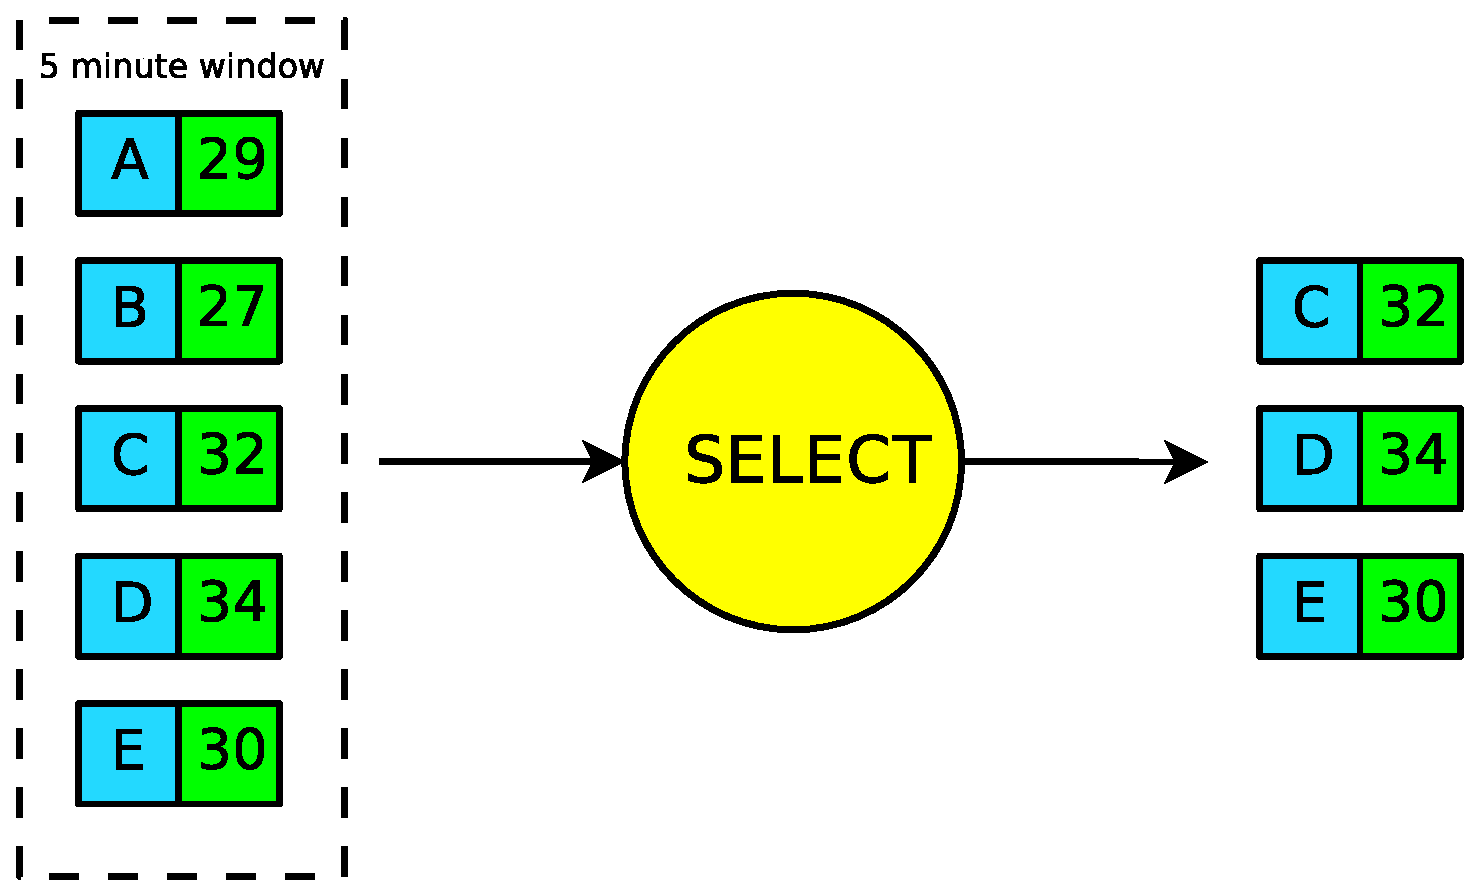
\includegraphics[width=0.55\textwidth]{img/tesi/cql-example} %XXX: rifare figura
	\caption{This query outputs all tuples with a temperature reading $\geq$ 30 in the last five minutes.}
	\label{fig:cql-example}
\end{figure}
\vspace{15pt}
\underline{\textsc{Example}}: Figure~\ref{fig:cql-example} illustrates a simple CQL query implementing
our temperature monitoring scenario. It signals all rooms, in which a temperature above 30~degrees
Celsius is detected in the past 5~minutes. The input stream is called \textsc{RoomTmpStr} and carries
tuples formed by a room identifier (\textsc{RoomId}) and a temperature reading (\textsc{RoomTmp}). A time-based window
is applied to it to obtain a snapshot that contains only fresh measurements generated in the past five
minutes. Once this relation has been created, a conditional \textsc{Select} is used to filter
out all tuples with a temperature value lower than 30~degrees. Finally, a new stream called
\textsc{HotRoomsStr} is created by an \textsc{IStream} relation-to-stream operator, containing tuples
from overheated rooms, which are then sent to control the air conditioning subsystem.\\
\tab \textsc{Select IStream(*)} \\
\tab \textsc{From RoomTmpStr[Range 5 Min]} \\
\tab \textsc{Where Tmp > 30} \\
%\clearpage
\vspace{-25pt}
%BOXES AND ARROWS
\subsection*{Boxes-and-Arrows Model}
\label{boxes_and_arrows}
A different paradigm to express queries over streams is the
\emph{boxes-and-arrows} model~\cite{boxes-and-arrows}.
It was introduced as part of the project Aurora~\cite{aurora-and-medusa} and also employed by
Borealis~\cite{borealis-design}.
In this model, a query is represented graphically as a data flow graph. Operators are depicted as boxes,
with streams being arrows connecting them. Tuples flow in a loop-free, directed graph of processing
operations. Queries in this model are specified by composing the query plan using a graphical interface
or by employing a query language such as SQuAl (Stream Query Algebra).
Aurora employs its own set of primitive operators, even though many of these have equivalents in a
traditional relational query model.
In this model, we can divide operators into two main categories: stateless and
stateful~\cite{borealis-app-manual}.
\paragraph{Stateless operators.} Steteless operators do not need to store any information about previous
tuples in order to execute.
\emph{Map} is an example of such an operator. It transforms some attributes of a tuple by applying a
predicate. If we consider a tuple carrying a temperature reading, for example, a Map operator can be
used to convert the temperature field from degrees Fahrenheit to Celsius.\\
In the same category, there is also a \emph{Filter} operator. It can be seen as the equivalent of a
\emph{Select} in the relational model.
It applies predicates to each input tuple and includes them in an output stream if the predicate evaluates to \emph{true}.
A Filter operator can have multiple output streams, depending on the number of specified predicates. \\
\emph{Union} is a simple operator that produces a single output stream from many input streams with the
same schema. The operator itself does not modify the tuples but it simply merges
streams. For example, it is used to provide a single stream as an input to other
operators, such as an Aggregate or a Filter.

\paragraph{Stateful operators.} Stateful operators maintain internal state, which is determined by the
tuples processed previously. 
In the boxes-and-arrows model, there is no explicit concept of a \emph{window} operator, unlike in CQL.
Instead, some operators are designed to support windowing on their input streams. The semantics for
expressing these windows are rich, and it is possible to state a wide range of windows, such as
count-based, time-based and partitioned. A sliding parameter can be used to specify the updating policy
of the window.\\
\emph{Aggregate} is a typical example of such an operator. It computes an aggregate function, such as a
sum or an average, over a window of tuples. A wide range of aggregate functions is provided, and others
can be specified by the user. It accepts a single input stream and is usually preceded by a Union operator. 
\emph{Join} is another classical stateful operator with two input streams and two windows. Join pairs
tuples from the two input windows that satisfy a given predicate, resembling its
relational~counterpart.\\
A special kind of stateful operators are synchronisation operators. This class includes \emph{Lock,
Unlock} and \emph{WaitFor}. These are used to buffer tuples temporarily until a certain condition is
reached.
\vsp
\paragraph{\mbox{Load-shedding} operators.} Load-shedding operators are used to overcome overload
conditions. They reduce the load of an operator by discarding a portion of its input. This category includes RandomDrop and
WindowDrop. \emph{RandomDrop} randomly discards a certain fraction of a stream. Every time the operator
is scheduled, it discards a number of tuples on its input window at random according to specified
dropping parameters. \emph{WindowDrop} allows for a more sophisticated specification of the windowing
parameters. Once a window has been computed, it chooses probabilistically if it should be kept or
discarded as a whole according to a dropping parameter.\\

% In Borealis, some other operators have been introduced to deal with fault-tolerance~\cite{revision-processing}. 
% As better described in Section~\ref{sec:borealis}, Borealis aims at eventual consistency, meaning that, once the system has recovered from failure, 
% it will try to replay some tuples and eventually correct its previously tentative results. \emph{RevisionJoin, RevisionAggregate} and \emph{RevisionFilter} are examples of operators used for this operations. Furthermore, replication can be employed to improve the dependability of the system. This means that
% some subsets of the query plan, called replica sets, are run in parallel at different sites, so that if a crash should happen at the processing node hosting a set of replicated operators, the system can continue to operate using the output of another replica set. When working with replication, some of the operators have to be substituted by their deterministic version, which only forward tuples coming from one replica set, usually the first ones to arrive. These operators have the same name as their traditional counterparts, with the difference of an initial $S$, for instance \emph{SUnion, SFilter} and \emph{SJoin}. 
% When employing these operators, replicas are actively competing to deliver results as soon as possible, improving non only enhancing the availability of the system but also improving its performance in terms of end-to-end latency~\cite{borealis-fast_and_reliable, borealis-fast_and_ha}.
\begin{figure}[b]
    \centering
    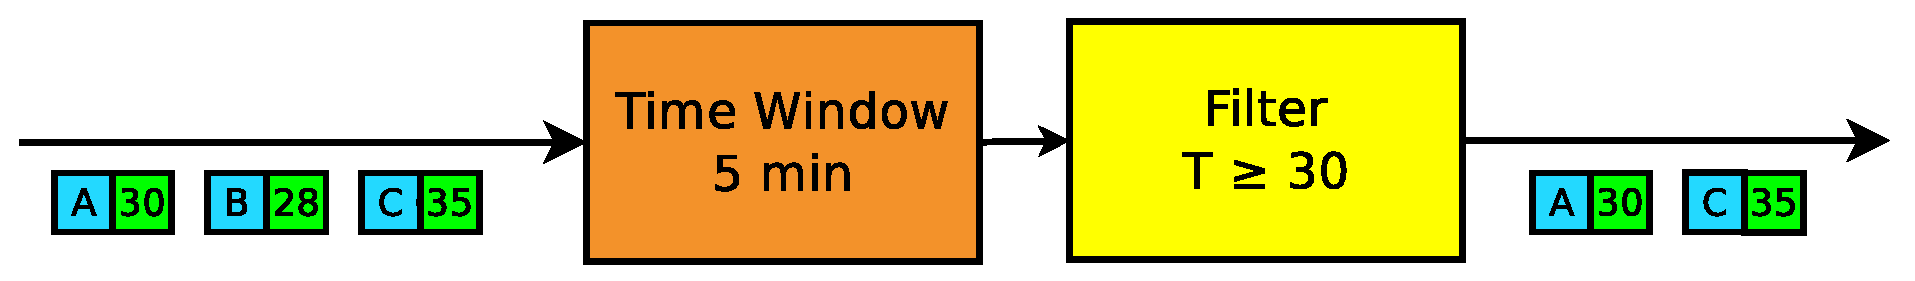
\includegraphics[width=0.8\textwidth]{img/tesi/baa-example}
    \caption{Temperature monitoring query example, expressed in the boxes-and-arrows model.}
    \label{fig:baa-example}
\end{figure}
\underline{Example:}\\
In the boxes-and-arrows model, implementing our temperature monitoring query is simple. 
Figure~\ref{fig:baa-example} shows the graphical representation of this query.
In this case, the query plan is composed only of a \emph{Filter} operator. It receives the stream of 
readings as input and outputs all tuples satisfying the predicate T $\geq$ 30. 




%--------------------------------------------------------------------------------------------------------

\section{System Model}
%  \bul{How does a stream processing system operates?} %\incite{8-reqs} %\incite{design-principles}   %
% %dbms vs DSPS Data stream processing systems (DSPS) compute real-time queries over constantly changing
% streams of data. A stream is a possibly infinite sequence of tuples, or timestamped entities.
% Differently than traditional databases, where queries are issued over stored data, in DSPSs queries are
% first submitted to the system, and results are generated continuosly as the new data enters the system
% in the form of streams. This allows the generation of real-time updated results based on the constantly
% changing available data streams.

% sp characteristics
Data Stream Processing Systems (DSPS) have been developed to process large volumes of stream data,
generated in real-time with new values constantly being introduced by the system. Using a traditional
approach of first storing the data and then executing the queries is not appropriate.
The first reason is the amount of available data~\cite{design-principles, 8-reqs}, which is typically
high and potentially too large to be stored entirely by the system.
Another reason not to store all the incoming data is related to its nature: often only a subset of
the data streams are relevant to the application.
Moreover, stream data is transient, with new values constantly updating old ones and rendering
them irrelevant.
Finally, data stream processing also has strict latency constraints and processing data streams with low
latency may be important. Storing the data before processing introduces an unacceptable
delay due to the latency cost of storing and retrieving data on disk.

Figure~\ref{fig:dbms+dsms} shows the two different architectures of a traditional
DBMS (left image) and a DSPS (right image). In the DBMS, queries are issued over previously stored data.
Since the data is already in the system, it is possible to create indexes over it in order to reduce the
query execution time. Results are generated from data received by the system \emph{up to the time} when
the query was issued. The picture on the right, instead, depicts a DSPS. Queries are issued over a
continuously changing stream of data. Once the data enters the system, it is matched against the
registered queries to produce the results. Results are generated from the data received by the system
starting \emph{from the time} when the query was first registered.

\begin{figure}[t!] \centering 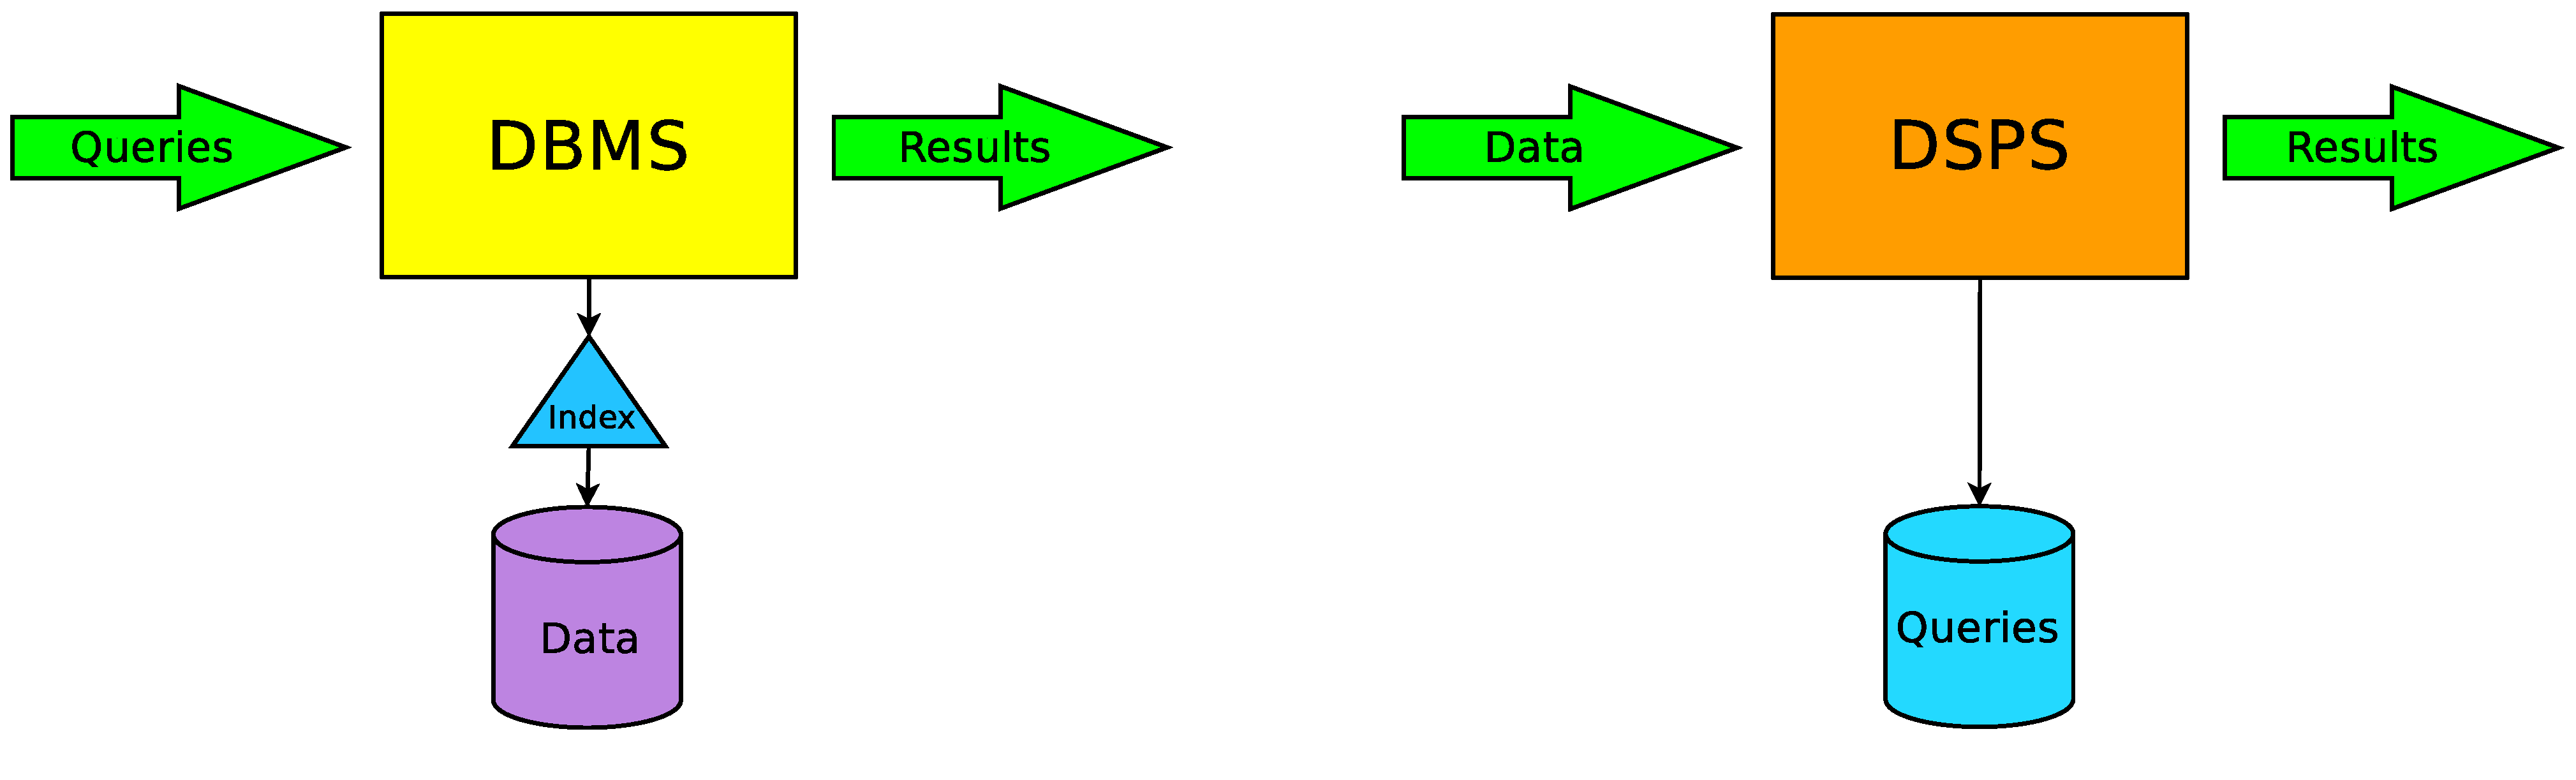
\includegraphics[width=\textwidth]{img/tesi/dbms+dsms} \caption{Comparison
between a traditional Data Base Management System (DBMS) and a Data Stream Processing System (DSPS). On
the left, queries are issued over stored data, while, on the right, data flows through continuous
queries.}
\label{fig:dbms+dsms}
\end{figure}

% \subsubsection*{Issues and Challenges}  \incite{stream-processing-challanges}
% \incite{ds-models-and-issues} \incite{dsm-issues}  \gap
\subsection*{Centralised Architectures}

The first generation of stream processing systems was centralised, with one processing node handling all
the computation. Examples of such systems are STREAM and Aurora.

STREAM~\cite{stream, stream-babcock, stream-chains} is a centralised DSPS, which tries to address the
issue of long-running continuous queries. It uses the relational Continuous Query
Language~(CQL)~\cite{cql} and supports SQL-like queries over continuous data
streams (see~Section~\ref{sec:cql}).
Once a query is registered in the system, a corresponding \textit{query plan} is derived from it.
Query plans are composed of \textit{operators}, which perform the actual processing, \textit{queues},
which buffer tuples as they move between operators, and \textit{synopses}, which store operator state.
All queries are expressed in CQL and then converted into an actual query plan which consists of these
basic elements.
In contrast Aurora~\cite{aurora} introduced the boxes-and-arrows model for queries. Operators are
regarded as boxes, with an input, an output and a specific processing semantic. They are linked
together by arrows representing the stream of tuples flowing between them.
			
\subsection*{Distributed Architectures}
% good replication
The natural step in the evolution of DSPSs is distribution. Centralised systems are inherently subject to
scalability issues. Distributing the processing over a number of nodes is the logical
approach to overcome this issue.
Distribution also allows for better dependability because operators can be replicated at different
locations, thus increasing availability. Fault-tolerance can also be achieved better by employing
distribution because different replicas of operators can be deployed, which achieves resilience to
failure.
The overall performance of the system is also increased by this approach because the computation can be
partitioned and run in parallel at different computing nodes. \\
Distribution can be realised at different scales. Processing nodes can be located within the same data
centre, taking advantage of the high bandwidth and low latency typical of these environments, or spread
out over wide-area networks to push scalability even further.

% issues
Distribution presents several advantages but it comes at a cost. Many issues arise when the system
is distributed: the operational complexity of the system increases and resources need to be allocated
efficiently. In a DSPS, distribution is achieved by partitioning the query plan and running clusters of
operators at different sites. Placing these operators correctly at deployment time and moving them at run time to rebalance the
system are not easy tasks. Running replicas can help increase the dependability of
the system but their correct management represents a key issue.

% systems
Building on the experience of Aurora, a centralised DSPS, other systems have been developed to explore
the possibilities offered by distribution. Aurora*~\cite{aurora*} is an evolution of the Aurora system
that provides interconnection among multiple Aurora instances running in a cluster environment.
A similar example is Medusa~\cite{aurora-and-medusa}, which expands the boundaries of
distribution outside a single cluster onto different processing sites administered by different
authorities.
Borealis~\cite{borealis-design} realises these experiences into a complete distributed
stream processing system. Borealis has been used to explore many research questions related to resource
allocation, \mbox{load-shedding} and replica management. In the following sections, we cover these
topics in more detail.
%  \incite{borBoreealis-design} \incite{mortar-short} \incite{mortar-long} \incite{ss-spc}
\vspace{-10pt}
\subsection*{Operator Placement and Load Balancing}
% op placement is difficult
The optimal distribution of streaming operators over a number of machines is key to maximise the
performance of a distributed stream processing system. Once a query plan has been divided into
clusters, these need to be mapped to available physical computing sites. A placement algorithm
assigns operators to processing nodes while satisfying a set of constraints and attempts to optimise some
objective function. Finding the optimal assignment among the total possible assignments is an NP-hard
problem and thus computationally intractable~\cite{npc-placement}. Despite this, many strategies have
been devised for efficient operator placement and, depending on the assumptions and requirements of the
system, different approaches are more suitable than others. A taxonomy of various placement strategies
for operators can be found in~\cite{placement_strategies}.

% load-balancing
Closely tied to operator placement is the problem of load balancing. While the former is more concerned
with the placement at deployment time, load balancing has to deal with the movement of operators at run
time. During the execution of a query, the amount of data carried by a stream can greatly vary. This may
result in computational overload at some nodes. To recover from this overload condition, the system can
decide to migrate certain operators to a better location, attempting to balance the load among the
available resources. Many operator placement algorithms recognise the need for placement reconfiguration
at run time and make load balancing a key component of their strategy.

% centralized
When the processing nodes of a DSPS are located within the same data centre, the topology management can
be performed by a centralised placement controller. In such environments, the controller can be
aware of the current state of the entire network, including workload information and resource
availability. Having access to this information allows it to reason about placement choices, with results
that are potentially optimal for small deployments. When the number of available resources becomes large
though, such an approach suffers from low scalability. Abadi et al.~\cite{borealis-design} describe
an approach which assumes a fairly constant workload and a heavy cost for operator migration. Xing et
al.~\cite{borealis-xing_placement} consider the workload to be highly unpredictable, thus requiring load
balancing at runtime. They also acknowledge the importance of initial placement and assume a high
migration cost for operators, thus developing an algorithm resilient to load variations~\cite{borealis-load}.
All these algorithms have been implemented within the Borealis DSPS.

% decentralized
When processing nodes are distributed over wide-area networks, a central coordinator becomes
ineffective and a decentralised approach to the problem is more appropriate. Such algorithms make
decisions based on local workload and resource information. Pietzuch et al.~\cite{sbon} propose a
distributed algorithm based on spring relaxation, to minimise a global metric called network usage based
on both bandwidth and latency. Another approach has been taken by Amini et al.~\cite{extreme-scale-sps}.
In this case, an algorithm maximises the weighted throughput of processing elements, while ensuring
stable operation in the face of highly bursty workloads. Zhou et al.~\cite{placement-zhou} propose an
algorithm, in which the initial deployment is determined through minimisation of the communication cost
among processing nodes. It then adapts to the changes in the data and workload within the system. Ying
et al.~\cite{placement-ying} propose to account for the state of operators when performing migration
decisions. When the resources are administered by multiple authorities, the degree of trust and
collaboration among them must be taken into account.
The algorithm from Balazinska et al.~\cite{medusa-load} achieves this by means of pre-negotiated
load-exchange contracts between nodes.
% \subsection*{Resource Allocation}  \subsubsection*{Cluster} \incite{placement-ying}
% \incite{placement-zhou} \incite{borealis-xing_placement} \incite{borealis-load_management}
% \incite{borealis-load}
% 					\incite{medusa-load}
% 					\incite{partial-fault-tolerance}
% 					
% \subsubsection*{Wide-Area}
% 
% 					\incite{sbon}
% 					\incite{placement_strategies} 
% 					\incite{streamglobe}
% 					\incite{adaptive-overlays}
% 					\incite{adaptive-query-deployment}
% 					\incite{adaptive-tree-reorganization}


%-------------------------------------------------------------------------------------------------------- 
       
\section{Overload Reduction}

When the rate of input data exceeds the processing capabilities of a node, the system becomes overloaded
and needs to take action. The rate of input data can vary rapidly, sometimes growing by orders of
magnitude, and the resource provisioning of the system thus quickly becomes inadequate. Scaling the
processing resources is not always feasible or cost effective. In order to overcome an overload
condition, it is possible to employ either \emph{\mbox{load-shedding}} (\ie the deliberate discarding of
a fraction of the input data), or \emph{approximate operators}, which produce a semantically similar
output but with a lower CPU or memory footprint. Next we describe each of these two approaches in turn.

\subsection*{Load-Shedding}

The discarding of a certain amount of input data is referred to as
\emph{load-shedding}~\cite{load-shedding}. The need to shed load comes from the inability of the system
to process all the incoming data tuples in a timely fashion. If the system is not able to sustain the
incoming rate of data with its processing throughput, the internal buffers holding the tuples awaiting
to be processed grow in size, leading to an increased latency of the result tuples and eventually to an
exhaustion of buffer memory. The most important choices that a system faces when overloaded are about (a)
the amount of tuples to discard, (b) where to discard tuples in order to maximise the impact of the
shedding and (c) what tuples to discard.
%--------------------------------------------------------------------------------------------------------
\subsubsection*{Overload Detection} 
In order to detect an overload condition, the system has to continuously monitor its input rate and the
size of its internal buffers. This periodic self-inspection has to be performed frequently enough so that
the system can promptly react to a sudden variation of input rates, while avoiding an excessive overhead
from the monitoring process.

Aurora~\cite{load-shedding} evaluates load based on a calculation that takes into account the
processing cost of operators and their selectivity. It assumes a query network $N$, a set of input
streams $I$ with certain data arrival rates and a processing capacity $C$ for the system that executes
$N$.
Let $N(I)$ denote the load as a fraction of the total capacity $C$ that network $N$ exerts on the
system.
An overload condition is detected when $Load(N(I)) > H \times C$, where $H$ is constant called the
\emph{headroom factor}. The total load calculation is a summation of the individual load
of all network inputs. Each input has an associated \emph{load coefficient}, which represents the number
of CPU cycles required to transfer a single tuple across the entire local operator graph. By observing
the input rates, it is possible to calculate if the current load leads to an overload condition and
trigger the \mbox{load-shedding} mechanism when needed. 
%--------------------------------------------------------------------------------------------------------
% 
% \subsubsection**{\mbox{load-shedding} Amount}
% When the system detects an overload condition, it first have to estimate what is the percentage of the
% current input that it needs to discard. It has to estimate what is the maximum sustainable throughput
% without an excessive increase in latency and without exhausting all the memory resources.
% 
% In STREAM~\cite{stream} the load of the processing node is constantly monitored by the \emph{StreaMon}
% component. 
% 
% 
% In Aurora~\cite{\mbox{load-shedding}} 
% 
% \gap
% %--------------------------------------------------------------------------------------------------------

\subsubsection*{\mbox{Load-Shedding} Location}

After an overload condition has been detected, the system has to choose the location, at which it is best
to discard the input data. In general, it is better to shed tuples before they are processed so that no
CPU cycles are wasted processing data that will be discarded. For some classes of
applications though, it may be better to perform the load-shedding at different locations, as explained
below.

Babcock et al.~\cite{loadshed-babcock} propose random drop operators, carefully inserted along a
query plan, such that the aggregate results degrade gracefully.
If there is no sharing of operators among queries, the optimal solution is to introduce a \mbox{load-shedding}
operator before the first operator in the query path for each query. Introducing load-shedding as early
in the query path as possible reduces the effective input rate for all downstream operators and conforms
to the general query optimization principle of ``pushing selection conditions down''.
In the case of shared streams among queries, the authors provide an algorithm that chooses the location
and the sampling rate of the \mbox{load-shedding} operators in an optimal way.

Tatbul et al.~\cite{loadshed-tatbul2} show that arbitrary tuple-based load-shedding can cause
inconsistencies when windowed aggregation is used. They propose a new operator called \emph{WinDrop}
that discards entire windows. The idea behind this approach is that
placing a tuple-based \mbox{load-shedding} operator before an aggregate does not reduce the load for the
downstream operators because the aggregate still produces tuples at the same rate. Placing the \mbox{load-shedding}
operator after the aggregate, instead, is not effective in reducing the system load either, because all
tuples are still processed and aggregate values are computed just to be discarded. Following this
reasoning, the WinDrop operator is designed to operate on the window of tuples to be sent to the
aggregate operator and discards or forwards this set of tuples as a whole.
%--------------------------------------------------------------------------------------------------------
\subsubsection*{\mbox{Load-Shedding} Selection}
Another important aspect of load-shedding is the correct selection of tuples to be discarded. The
simplest approach is to discard the required amount of tuples at random, avoiding a selection step in
the load-shedding algorithm. In contrast, choosing a specific set of tuples according to some
criteria allows the implementation of \emph{semantic shedding strategies} that can improve the quality of
the computed results. Such approaches have been used, for example, in the context of aggregate
queries and streams presenting irregular frequency patterns.
	
Mozafari et al.~\cite{loadshed-mozafari} propose an algorithm for optimal \mbox{load-shedding} for
aggregate queries when queries have different processing costs, different priorities and, importantly,
the users provide their own error functions. \mbox{Load-shedding} is treated as an optimisation problem,
in which users state their needs in term of quality-of-service requirements, \eg the maximum error
tolerated. The system then implements a shedding policy that meets those requirements. If the minimum
quality of the results cannot be achieved for a query with the available resources, all inputs for that
query are discarded, and the freed resources are allocated to the other remaining queries. Using this
approach, the user has to choose among \emph{approximate} and \emph{intermittent} results. The most
demanding queries in terms of processing capacity tend to deliver intermittent results because all their
data is discarded frequently; small lightweight queries tend to deliver approximate results due to
a partial loss of their input data.

Chang et al.~\cite{loadshed-chang} propose an adaptive \mbox{load-shedding} technique based on the
frequency of input tuples. 
In many data stream processing applications, such as web analysis and network monitoring,
where the aim is to mine frequent patterns, a frequent tuple in the data stream can be considered
more significant compared to an infrequent one. 
Based on this observation, frequent tuples are more likely to be selected for processing while
infrequent tuples are more likely to be discarded.
The proposed technique can also support a flexible trade-off between the frequencies of the
selected tuples and the latency defined as the delay between the generation and processing time.
One of the proposed algorithms, in fact, buffers tuples for a certain amount of time so that the
\mbox{load-shedding} decision can be made based on the frequency of tuples over multiple time slots.

\subsubsection*{Distributed \mbox{Load-Shedding}}
In a distributed stream processing system, every node acts as an input provider for its downstream nodes.
The reduction of load at a node thus also reduces the amount of load on all other nodes hosting the
subsequent operators in the query graph. This makes the problem of identifying the correct
\mbox{load-shedding} plan more challenging than in a centralised environment. 

In the Borealis system~\cite{borealis_load_management}, the \mbox{load-shedding} problem is solved using
linear optimisation.
The goal is to maximise the output rate at the query end-points. The system inserts a number of
\mbox{load-shedding} operators and chooses their drop selectivities, the percentage of tuples to be
discarded, so that the total throughput is maximised. The solution of the \mbox{load-shedding} problem is broken down into
four steps: (i) advanced planning; (ii) load monitoring; (iii) plan selection; and
(iv) plan implementation. In the first step, a series of \mbox{load-shedding} plans is computed, one for each
predicted overload condition. Then, during the lifetime of the query, the load is monitored at
each node. When an overload condition is detected, one of the previously computed shedding plans is
selected and implemented at the various nodes, adding the corresponding set of \mbox{load-shedding}
operators. The idea is to prepare the system against all possible overload conditions beforehand and to
modify the query at run-time depending on the expected overload scenario. This general approach has been
implemented in two ways: in a \emph{centralised} and in a \emph{distributed} fashion.

\paragraph{Centralised Coordination.} In the centralised approach, a central server called the
\emph{coordinator} is used to calculate all the \mbox{load-shedding} plans. It uses information obtained from all processing nodes
about the operators they are hosting, their input rates and their selectivities. Based on this
information, it generates a number of \mbox{load-shedding} plans to address various overload scenarios.
Once the plans are generated, they are passed to the processing nodes. The
coordinator then starts monitoring the processing load at each node. If an overload condition is
detected, the coordinator selects the most suitable plan to address it and triggers its execution at the
processing node.

\paragraph{Distributed Coordination.} In the distributed approach, the four \mbox{load-shedding} steps
are performed cooperatively by all the processing nodes, without the help of a centralised coordinator. All nodes
communicate with their neighbours and propagate information about their input rates and processing
capabilities. Each node identifies a feasible input load for itself and all its downstream neighbours.
This information is used to compute a \emph{Feasibility Input Table (FIT)}, a table containing
the input rate combinations that are feasible (\ie not causing overload) for that node.
Once a node has calculated its FIT table, it is propagated to its parent nodes. The parent node
aggregates the FITs of all children and eliminates those that are infeasible for itself. The propagation
continues until the input nodes receive the FITs of all their downstream nodes. At this point, when an
overload conditions arises, every node is able to select a \mbox{load-shedding} plan among those
contained in its FIT, reducing the load for itself and all its downstream nodes.
% 
% 			\incite{borealis-load}
% 			\incite{borealis-load_management}
% 			\incite{\mbox{load-shedding}}
% 			\incite{loadshed-babcock}		AGGREGATE
% 			\incite{loadshed-chang}		S	FREQUENCY BASED
% 			\incite{loadshed-chi}		S	CLASSIFICATION
% 			\incite{loadshed-dash}		S	XML
% 			\incite{loadshed-gedik}		S	non-uniformly regulated sifters, 
% 			
% 			\incite{loadshed-gedik2}
% 			\incite{loadshed-grubjoin}
% 			\incite{loadshed-kendai}	S similar to aurora, drop around the mean
% 			\incite{loadshed-mozafari}
% 			\incite{loadshed-tatbul}
% 			\incite{loadshed-tatbul2}
% 			\incite{loadshed-telegraphcq}
% 			\incite{loadshed-tu}
\subsection*{Approximate Operators} 
Overload can also occur when the total state of all running operators exceeds the available memory. 
In this case, the system has to reduce the memory usage by reducing the state kept by operators. 
In general, the system can try to minimise its memory footprint through a number
of techniques.
For example, it can exploit constraints on streams to reduce state either by letting the user specify
them or by inferring them at run-time. It can also \emph{share state} among operators when they materialise nearly
identical relations.
It can also schedule operators intelligently in order to minimise the length of queues in
memory~\cite{stream-chains}.
While these techniques do not lower the quality of the processing, the memory usage may still exceed the
limits of the systems. In such situations, the internal state of operators can be approximated. In the
case of aggregation and join operators, the state can be reduced by employing sampling techniques, such
as using \emph{histograms}~\cite{histograms}. These are approximations to data sets, achieved by
partitioning the data into subsets, which are in turn summarised by aggregate functions. Every column in the histogram is a compact
representation of one of these subsets. Another summarising technique that can be employed makes use of
wavelet synopses~\cite{wavelets}. For set difference, set intersection and duplicate
elimination operators, Bloom filters can be employed~\cite{bloom}. These are compact set representations
that provide a fast way of testing whether an element is a member of a set. All these techniques trade
memory usage against precision and can greatly help the system overcome or avoid memory-induced overload
conditions.



%--------------------------------------------------------------------------------------------------------    

\section{Failure}

In a large-scale distributed stream processing system, failure should not be considered a rare, transient
condition. The previous section described failure due to overload (\ie when the system resources are
insufficient to carry out perfect processing). Failure, however, can also occur for other reasons.
When dealing with a large number of processing units, it is not uncommon for a node to crash, thus leading to
the partial disconnection of the query graph. It is also possible that a processing node becomes
temporarily unreachable because of a network partition, especially in a widely geographically distributed processing
infrastructure. 

A stream processing system should address such issues in order to achieve a high level of dependability.
The term dependability~\cite{dependability} in this context refers to the ability of a system to
withstand failure and to efficiently recover from it. It should choose an appropriate \emph{consistency
model}, a contract with the user stating how failure will be handled, and employ a \emph{replication
model} to be more resilient to the occurrence of failure.

\subsection*{Consistency Model}
When failure occurs in a stream processing system, a choice arises between stopping the delivery of
results while recovering or delivering incorrect results. In the first case, the \emph{availability} of
the system is reduced because no results are produced during the recovery phase; in the latter case it
is the \emph{consistency} of results that is compromised. The system can also opt for a hybrid
approach~\cite{availability-consistency} delivering first imperfect results, marking them as
``unstable'', while trying to correct them as soon as the failure has been overcome. This model is called
\emph{eventual consistency} because eventually all the delivered results will be correct.
Another approach, called \emph{relaxed consistency} is to avoid correcting results and instead trying to
augment them with a metric quantifying the amount of failure incurred~\cite{dependable-is-sensing}.
This approach has been adopted in this thesis because we consider failure a constant
operating condition of the system and the cost to achieve eventual consistency would become too high to
be acceptable.
			
Borealis~\cite{borealis-fault_tolerance} adopts a strict consistency model that aims at eventual
consistency. This means that in the case of tuple loss or misordering, the system tries to obtain
the correct final result. It achieves this by marking a stream on which an error has
occurred as \emph{tentative}.  Later the system attempts to restore the correct result by employing
a revision process, which ensures that the final result is correct.  Of course, this assumes a
scenario in which a fault is more an exception than the rule, as the cost for the revision process can
become high. There is no mechanism to quantify the input of the fault to the user. As the fault is
thought to be transient and recoverable the only feedback given to the user is that the stream content is
invalid and cannot be trusted until recovery. Instead, we propose a quality-centric data model that
allows the system to quantify the impact of the error and to provide the user with feedback on the
actual processing quality of the system.\\
The revision mechanism used in Borealis also supports ``time travel''.  It is possible to recalculate
tuples for the past and even in the future (by providing a prediction formula).
Rolling back processing to the past is a heavy-weight process and requires a large
amount of storage, which is not always feasible in stream processing.\\
Figure~\ref{fig:borealis-fault_tolerance} shows the state machine for the fault tolerance mechanism
employed by Borealis. When failure occurs upstream in the query graph, an operator is alerted by the
arrival of tentative tuples or by the lack of heartbeat messages.
It then marks its tuples as tentative while waiting the restoring of a stable
state for the processing. When failure has been overcome, the state is reconciled and the system
becomes stable once again.

\begin{figure}[t] 
	\centering
	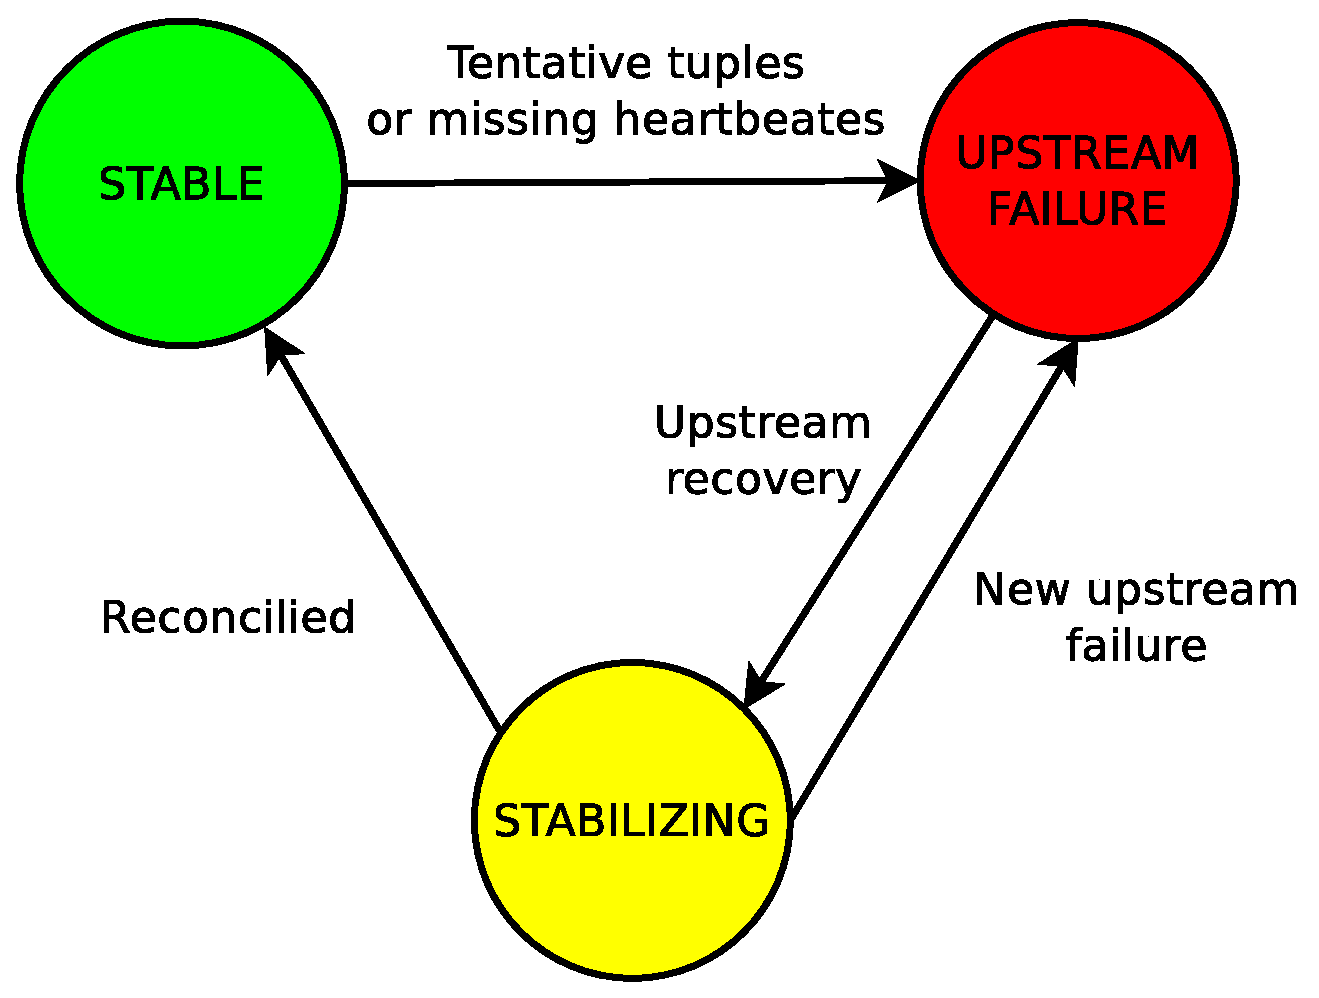
\includegraphics[width=.4\textwidth]{img/tesi/borealis-fault_tolerance}
	\caption{State machine describing Borealis fault tolerance mechanism in Borealis. }
\label{fig:borealis-fault_tolerance}
\end{figure}

In the relax consistency model proposed by Murty and Welsh~\cite{dependable-is-sensing}, operators are
considered to be \emph{free-running}, updating their internal state independently as incoming tuples
arrive. This means that two replicas of the same operator may produce different outputs because of their
different internal state due to failure.
Instead of trying to achieve eventual consistency, they propose to
deliver imperfect results but augmenting them with two quality metrics called \emph{harvest} and
\emph{freshness}. These metrics provide the user with information about the quality of the results.
Harvest represents the coverage of a query result in terms of data sources. Its value is reduced by
failures during query processing. A harvest of 100\% indicates that the result was computed
using data from all sources.
This metric is not directly related to correctness but rather provides an indication of
the confidence the user should have in the delivered results. A high value for harvest means that
the provided result incorporates a large number of the input sources.
Freshness represents the age of the input data that generated the result. A high network latency or a
high system load affect the freshness value of the delivered tuples negatively. The lower bound for
freshness is the network latency.

	
\subsection*{Replication Models}

In order to be more resilient to failure, stream processing systems frequently employs \emph{operator
replication}.
The system identifies the most important operators in a query and runs multiple copies of them
concurrently.
In this way, if a node hosting a part of the query fails, one of its replicas can be used instead,
without any impact on the processing.
Replication is not only useful to increase the dependability of the system but it can also improve its
performance by running the replicas in competition in order to reduce
latency~\cite{borealis-fast_and_ha, borealis-fast_and_reliable}.

%borealis
Early work on replication in a DSPS have been focused on masking software
failures~\cite{borealis_ha_algos} by running multiple copies of the same operators at different nodes.
Others~\cite{ha_ft_dataflows} proposed to strictly favour consistency over availability by
requiring at least one fully connected copy of the query graph to be working correctly in order for the
computation to proceed. %\\
In Borealis, the approach has been to provide a configurable trade-off between availability and
consistency~\cite{borealis-fault_tolerance}.
This is done by letting the user specify a time threshold, within which all tuples are processed
regardless of whether failures occurred or not on the input streams. This increases availability because
the operator continues to process even in the presence of failures on its input streams. Output tuples,
are then marked as \textit{tentative} in order to signal the incorrectness of the results. After the
system has recovered from the failure, it reconciles the state of operators that processed
tentative tuples, by re-running their computation with the stable data tuples. This also means that every
source or operator has to buffer all their outgoing tuples, at least for a certain amount of time, to
replay them in case of failure. The goal of Borealis is to achieve \textit{eventual consistency} and
provide all clients with complete correct results.

%murty&welsh
Another approach to the management of replicas has been proposed in~\cite{dependable-is-sensing}. The authors take a
different standpoint on failure by not considering it as an infrequent event but as a constant condition
of the system. In this case, maintaining consistency among replicas becomes even harder. The
authors claim that it is better to ignore this requirement and to employ \textit{free-running} operators
instead.
Operators are permitted to update their internal states independently as incoming tuples arrive. In case
of recovery from failure, for example, an operator restarts, without any knowledge of its
previous state. However, this means that an operator's state can diverge from its replicas due to
missing tuples.
In general, though, the state of an operator is based only on the tuples in its \textit{causality
window}. Thus, assuming a window size of $w$ seconds and no additional failure, the system will regain
consistency without the need for explicit synchronization. Whenever the replicas are out of sync and
produce different results, however, the system needs to choose, which set of results represents the
``best'' answer.
It can do so in several ways, for example, by choosing tuples generated by the replica with the largest
uptime, with a majority vote among the replicas, or by relying on some \textit{quality metric}
describing the quality of the data. This process is referred to as \textit{best-guess reconciliation}.


%--------------------------------------------------------------------------------------------------------					
\section{Summary}

This chapter presented the relevant background to understand the work presented in this thesis.
It started with a description of a range of stream processing applications, in particular those that have
to deal with large amount of data and can tolerate a certain degree of approximation in their results.
Environmental monitoring is crucial for the timely prediction of possibly disruptive weather phenomena
and for the long term understanding of world-wide climate change. Social media analysis deals with the
processing of user-generated content in online social networks, which is a valuable tool for researchers
to investigate the spread of information through social cascades.
We also presented the most important query models used to express queries in stream processing systems:
the continuous query language (CQL), which extends the relational model for the processing of unbounded
streams, and the boxes-and-arrows model, which employs a visual paradigm to compose queries by creating a
network of operators.
After that, we introduced a system model for stream processing, presenting examples of systems that
pioneered centralised as well as the distributed processing. When dealing with a distributed environment,
the correct allocation of resources across processing sites is crucial. In this regard, we described
efficient resource allocation techniques for both data centre and wide-area deployments.
A major focus of this work is on techniques for the management of overload, in particular
\mbox{load-shedding}.
An overview of the most relevant strategies to discard input data efficiently was provided emphasising
the different issues related to \mbox{load-shedding}.
Finally, there was a description of techniques used to avoid and recover from failures, with a discussion
on the possible consistency and replication models.\\
The next chapter will describe the data model developed in the scope of this thesis which includes a
quality metric that can be used to augment streams and allow the system to detect and measure the effect
of overload. 
	

